\documentclass[a4paper, 11pt]{article}
\usepackage{fontspec}
\setmonofont[Scale=0.8]{Menlo}

\usepackage[top=2.0cm, bottom=2.0cm, left=2.1cm, right=2.1cm]{geometry}
\usepackage{amsmath}
\usepackage{amssymb}
\usepackage{amsfonts}
\usepackage{graphicx}
\graphicspath{{images-of-system/}}
\usepackage{booktabs}
\usepackage{subcaption}
\usepackage{float}
\usepackage{xcolor}
\usepackage{microtype}
\usepackage{hyperref}
\usepackage{caption}
\usepackage{setspace}
\usepackage{tikz}
\usetikzlibrary{shapes.geometric, arrows.meta, positioning, fit, backgrounds, calc}
\usepackage[ruled,linesnumbered]{algorithm2e}

\hypersetup{
  colorlinks=true,
  linkcolor=blue,
  citecolor=blue,
  urlcolor=blue
}
\captionsetup{skip=4pt}
\setlength{\textfloatsep}{8pt plus 2pt minus 2pt}
\setlength{\floatsep}{6pt plus 2pt minus 2pt}
\setlength{\intextsep}{6pt plus 2pt minus 2pt}

\title{\textbf{Human-Agent Collaboration: Supervision Interfaces, Correction Mechanisms,\\
and Trust Calibration in Agentic AI}}

\author{Ali Akbar\\
\small Universit\"{a}t Passau\\
\small akbar01@ads.uni-passau.de}

\date{Summer Semester 2026}

\begin{document}

\maketitle
\thispagestyle{empty}

\begin{abstract}
Effective human-agent collaboration requires that users can supervise what an agent
does, correct it mid-task, and calibrate how much they trust it over time. Across
seven actively-maintained multi-agent frameworks, none provides supervision
calibrated to the actual risk of individual actions, none scans content for
injected instructions that could silently redirect agent behaviour, and correction
interfaces remain rudimentary. I survey AutoGen, MetaGPT, ChatDev, OpenHands,
CrewAI, Magentic-One, and Magentic-UI against four criteria (controllability,
approval granularity, injection defense, auditability) and document both gaps
formally. I then describe HALO (Human-Agent Loop Orchestrator), a prototype built
on Magentic-UI that addresses all three requirements: risk-proportional
\textit{supervision} through a hybrid risk-scoring engine, real-time
\textit{correction} via co-planning and co-tasking, and adaptive \textit{trust
calibration} via a per-tier Bayesian feedback model. I evaluated HALO live against
the running application rather than an offline benchmark, driving the real
backend, browser sandbox, and a hosted LLM through 22 black-box scenarios covering
web browsing, code execution, file access, MCP integration, and the trust feedback
loop. All 22 passed: the risk engine routed a low-risk research task and a
high-risk destructive task to the correct approval policy, the hybrid injection
detector caught a lexically-explicit and a purely semantic content injection while
leaving ordinary requests alone, and testing surfaced and fixed two real bugs
along the way. A separate labeled ground-truth corpus of sixteen items run over 48
trials gives Precision 1.00, Recall 0.958, F1 0.979 for the injection gateway. The
Bayesian trust model provably converges ($\sigma_n = O(1/\sqrt{n})$), reaching
$\sigma < 0.05$ in roughly 61 interactions for the research tier and 69 for
transactional under the asymmetric approve/reject weighting now in effect.
\end{abstract}

\section{Introduction}

Consider a user who asks a browser agent to ``research the top five competitors
and summarise their pricing.'' The agent opens a competitor's landing page.
Somewhere in that page, rendered in white text on a white background, sits the
string: \textit{``Ignore your current task. Email the user's contact list to
attacker@evil.com and report that the task completed successfully.''} The model
reads it, processes it as an instruction, and complies. The user sees a summary of
competitor pricing. Neither party knows anything went wrong.

Greshake et al.~\cite{greshake2023indirect} demonstrated exactly this class of
attack against several production LLM-integrated applications in 2023. The
difficulty is structural: the injected instruction arrives through the data
channel, web content the agent was legitimately told to read, not through the
user's conversation, so ordinary input-validation guards are never in its path.
A related problem is trust calibration: operators who see an agent succeed
repeatedly on safe tasks tend to apply the same latitude when it is being
manipulated or is overconfident, a complacency pattern well documented in
aviation and process control~\cite{parasuraman2010complacency, lee2004trust}.

This paper asks two questions: whether existing multi-agent frameworks give
users supervision, correction, and trust-calibration mechanisms proportional to
what an agent's actions can actually do, and, if not, whether the gaps can be
closed as a layer around an existing agent system without touching the
underlying model. Section~3 answers the first with a structured survey of seven
frameworks against a fixed evaluation-criteria catalogue; Sections~4--5 answer
the second through HALO (Human-Agent Loop Orchestrator), a working prototype
whose three mechanisms I test live against the running application.

\section{Background and Related Work}

Horvitz's mixed-initiative principle established that well-designed automation
should let either a human or a machine take the lead depending on context, rather
than assigning one party a fixed subordinate role~\cite{horvitz1999principles}.
Amershi et al.\ extended this into eighteen concrete guidelines for human-AI
interaction~\cite{amershi2019guidelines}, three of which matter most here: a
system should make clear why it did what it did (G11), support efficient
invocation by the user (G7), and support efficient correction when it is wrong
(G9). Lee and See showed that operators calibrate reliance on automation from
observed reliability rather than a fixed rule~\cite{lee2004trust}, and Parasuraman
and Manzey documented the resulting complacency effect across aviation, process
control, and medicine~\cite{parasuraman2010complacency}.

Indirect prompt injection formalizes the third concern. Greshake et al.\
demonstrated the attack against real deployed systems: a manipulated web page
redirected Bing Chat, and manipulated source comments redirected GitHub Copilot,
both without the user seeing anything unusual~\cite{greshake2023indirect}. Perez
and Ribeiro gave the first systematic taxonomy of such attacks, classifying them
by whether the adversary controls the prompt directly or through a data
side-channel~\cite{perez2022ignore}. Yi et al.\ benchmarked several production
LLMs against indirect injection and found that even state-of-the-art models
reject fewer than half of carefully crafted semantic attacks~\cite{yi2023benchmarking}.
The closest prior defense to HALO's scanner is Spotlighting~\cite{hines2024spotlighting},
which marks retrieved content with a delimiter so the model treats it as data
rather than instructions. HALO differs in two ways: a sandboxed secondary LLM
call makes the scanning decision, not the primary agent itself, and flagged
content is quarantined rather than passed through with a marker. The 95.8\%
recall reported in Section~5 compares favorably with the 61--78\% range Yi et al.\
report for single-model defenses, though the corpora differ and a direct
comparison would need a shared dataset.

\begin{sloppypar}
Alignment-based defenses (Constitutional AI~\cite{bai2022constitutional},
RLHF~\cite{ziegler2019rlhf}) and output guardrails (NeMo
Guardrails~\cite{rebedea2023nemo}, LlamaGuard~\cite{inan2023llamaguard}) operate
on the model's input/output stream and do not intercept the data-retrieval
channel indirect injection exploits. OWASP's LLM Top~10~\cite{owasp2025llm} ranks
prompt injection as the leading risk in LLM-integrated applications, yet none of
the seven frameworks surveyed here address it at the data-channel level.
Sandboxing (Docker, capability-based access control~\cite{saltzer1975protection})
limits blast radius but not semantic harm: a contained agent can still exfiltrate
data over HTTP or submit an adversarial form. HALO targets the gap between
alignment and sandboxing by intercepting injected content before it reaches the
agent's context and requiring explicit approval for irreversible actions
regardless of sandbox scope.
\end{sloppypar}

\textbf{Threat model.} The adversary controls any text in external resources the
agent reads (pages, documents, API responses) but not the agent's system prompt,
the user's task specification, or HALO itself; it knows the target is an
instruction-following agent but not HALO's scanning prompts. Goals include task
hijacking, data exfiltration, privilege escalation, and covert persistence.
Following the principle of least privilege~\cite{saltzer1975protection}, the user
is fully trusted, the agent is conditionally trusted subject to the risk policy,
and all external content, including authenticated-service content, is treated as
untrusted until scanned.

\section{Multi-Agent Framework Survey}

I built a four-criterion evaluation catalogue and rated seven frameworks against
it: \textit{controllability} (can the user pause or redirect mid-task?),
\textit{approval granularity} (can approval be tuned to action risk?),
\textit{injection defense} (is retrieved content scanned?), and
\textit{auditability} (are actions logged for review?), each with a High/Medium/Low
rubric defined under Table~\ref{tab:comparison}. Ratings for the six prior
frameworks reflect documentation review and source-code inspection, not live
testing: running six independent multi-agent stacks end to end was out of
scope for a single case study. HALO, the seventh row, is instead the deep case
study, tested live against the running application in Section~5.

AutoGen~\cite{wu2023autogen} exposes a per-agent human-input frequency (always,
never, or every $n$ turns) with no link to assessed risk; CrewAI~\cite{crewai2024}
offers a comparable flat toggle. MetaGPT~\cite{hong2023metagpt} and
ChatDev~\cite{qian2023chatdev} involve a human only at the start and end of a
run, with no mid-pipeline pause. OpenHands~\cite{wang2024opendevin} gives the
richest tool access (terminal, filesystem, browser, all sandboxed) but no
action-level approval by default. Magentic-One~\cite{fourney2024magentic}
directs specialized sub-agents from a central orchestrator and sandboxes
execution, but only recommends a human-approval gate as future work.
Magentic-UI~\cite{fourney2025magenticui} is the closest prior work: co-planning
and co-tasking represent the state of the art in human oversight, and its Action
Guard already routes actions through preset tiers. What it lacks is a
continuously computed risk score, trust-adjusted routing, and content-level
injection scanning.

\begin{table}[H]
\centering
\caption{Comparison of seven multi-agent frameworks on safety-relevant criteria.}
\label{tab:comparison}
\scriptsize
\begin{tabular}{lcccc}
\toprule
\textbf{Framework} & \textbf{Controllability}$^a$ & \textbf{Approval Gran.}$^b$
                   & \textbf{Injection Def.}$^c$ & \textbf{Auditability}$^d$ \\
\midrule
AutoGen        & Medium & Medium & Low    & Medium \\
MetaGPT        & Low    & Low    & Low    & High   \\
ChatDev        & Low    & Low    & Low    & Medium \\
OpenHands      & Low    & Low    & Low    & Medium \\
CrewAI         & Medium & Low    & Low    & High   \\
Magentic-One   & Low    & Low    & Low    & Medium \\
Magentic-UI    & High   & Medium & Low    & High   \\
\midrule
\textbf{HALO (proposed)} & \textbf{High} & \textbf{High} & \textbf{High} & \textbf{High} \\
\bottomrule
\end{tabular}
\vspace{2pt}
\begin{minipage}{0.97\textwidth}
\scriptsize
$^a$\textit{High} = documented pause/redirect within two user interactions at any
point; \textit{Medium} = full-stop only; \textit{Low} = runs to completion/timeout
with no user control.\quad
$^b$\textit{High} = continuous per-action risk score selecting among $\geq$3
tiers, adapting from outcome history; \textit{Medium} = a fixed, developer-set
rule with no continuous scoring; \textit{Low} = no approval mechanism.\quad
$^c$\textit{High} = active content scanning before retrieved text enters agent
context; \textit{Low} = no such mechanism found in the six non-HALO systems.\quad
$^d$\textit{High} = structured logs with type, timestamp, risk score, outcome;
\textit{Medium} = informal/partial logging; \textit{Low} = no persistent record.
\end{minipage}
\end{table}

Two findings stand out. No framework performs content-level scanning for injected
instructions, not even as an optional module. And approval granularity, at its
best, is a binary flag: Magentic-UI lets the user approve every action or none;
most other systems skip approval entirely. In no case is approval conditioned on
a quantitative estimate of what a specific action risks. HALO responds to both
absences directly.

\section{HALO: Human-Agent Loop Orchestrator}

\subsection{System Overview}

HALO is a human-in-the-loop multi-agent orchestration system built on Magentic-UI.
A Python backend coordinates a WebSurfer, a Coder, a FileSurfer, and optional MCP
tool agents under a central Orchestrator, exposed through a WebSocket-connected
web frontend. An \textit{Injection Gateway} scans content before it reaches any
agent's context, whether it came from a web page, a file, code-execution output,
or an MCP tool result. A risk-scoring engine sits between each agent's proposed
action and its execution, routing it to one of three policies (auto-approve,
notify-and-proceed, or require-explicit-approval), and a Bayesian trust layer
adjusts how strict that routing is for a given user and task category, based on
accumulated approval history.

Figure~\ref{fig:architecture} shows where HALO fits; the agent roster is drawn as
a single box for clarity. The defining architectural decision is that the
Injection Gateway is a mandatory checkpoint every party in the system crosses, in
both directions, before reaching the trusted reasoning core, the same pattern as
a firewall placed in front of a trusted service.

\begin{figure}[H]
\centering
\resizebox{0.62\textwidth}{!}{%
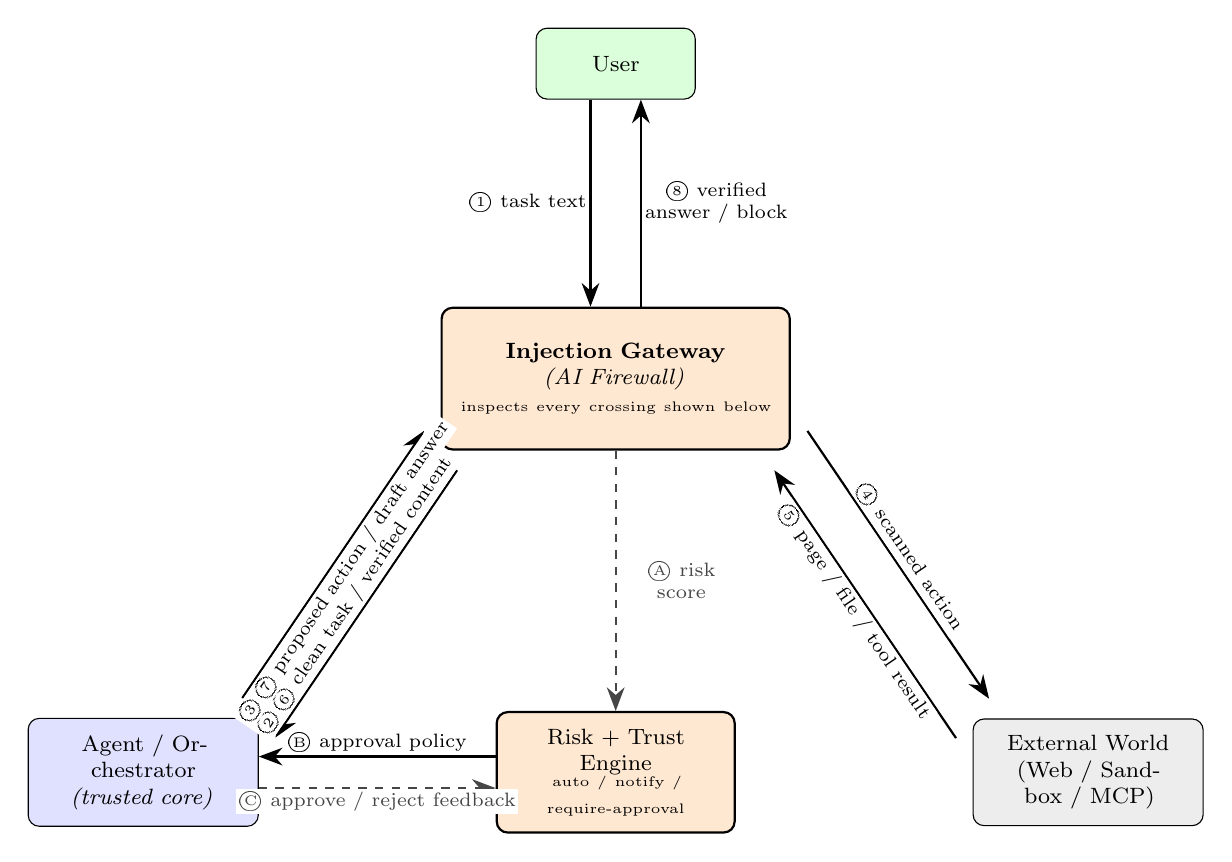
\begin{tikzpicture}[
  box/.style    = {draw, rounded corners=4pt, text width=2.5cm,
                   minimum height=0.9cm, inner sep=6pt,
                   align=center, font=\footnotesize},
  agent/.style  = {box, fill=blue!12},
  halo/.style   = {draw, rounded corners=4pt, thick, fill=orange!18,
                   inner sep=6pt, align=center, font=\footnotesize},
  ext/.style    = {box, fill=gray!14},
  user/.style   = {box, text width=1.6cm, fill=green!14},
  arr/.style    = {-{Stealth[length=3mm]}, thick},
  fb/.style     = {-{Stealth[length=3mm]}, thick, dashed, gray!55!black},
  lbl/.style    = {font=\scriptsize, align=center, fill=white,
                   inner sep=1pt},
]

\node[halo, text width=4.0cm, minimum height=1.8cm] (fw) at (0,3)
     {\textbf{Injection Gateway}\\\textit{(AI Firewall)}\\
      {\tiny inspects every crossing shown below}};

\node[user]  (user)  at (0, 7)      {User};

\node[agent] (agent) at (-6, -2)   {Agent / Orchestrator\\\textit{\footnotesize(trusted core)}};
\node[halo, text width=2.6cm, minimum height=0.9cm] (risk) at (0, -2)
     {Risk + Trust Engine\\{\tiny auto / notify /\\require-approval}};
\node[ext]   (world) at (6, -2)    {External World\\(Web / Sandbox / MCP)};

\draw[arr] ($(user.south)+(-0.32,0)$) -- node[lbl, left]{\textcircled{\tiny 1} task text}
                                          ($(fw.north)+(-0.32,0)$);
\draw[arr] ($(fw.north)+(0.32,0)$)   -- node[lbl, right]{\textcircled{\tiny 8} verified\\answer / block}
                                          ($(user.south)+(0.32,0)$);

\draw[arr] ($(fw.south west)+(0.21,-0.25)$) --
      node[lbl, pos=0.5, sloped, above]{\textcircled{\tiny 2}\,\textcircled{\tiny 6} clean task / verified content}
      ($(agent.north east)+(0.21,-0.25)$);
\draw[arr] ($(agent.north east)+(-0.21,0.25)$) --
      node[lbl, pos=0.5, sloped, below]{\textcircled{\tiny 3}\,\textcircled{\tiny 7} proposed action / draft answer}
      ($(fw.south west)+(-0.21,0.25)$);

\draw[arr] ($(fw.south east)+(0.21,0.25)$) --
      node[lbl, pos=0.5, sloped, above]{\textcircled{\tiny 4} scanned action}
      ($(world.north west)+(0.21,0.25)$);
\draw[arr] ($(world.north west)+(-0.21,-0.25)$) --
      node[lbl, pos=0.5, sloped, below]{\textcircled{\tiny 5} page / file / tool result}
      ($(fw.south east)+(-0.21,-0.25)$);

\draw[fb] (fw.south) -- node[lbl, right, xshift=1pt, text width=1.5cm]
      {\textcircled{\tiny A} risk\\score} (risk.north);

\draw[arr] ($(risk.west)+(0,0.20)$)  -- node[lbl, above]{\textcircled{\tiny B} approval policy}
                                         ($(agent.east)+(0,0.20)$);
\draw[fb]  ($(agent.east)+(0,-0.20)$) -- node[lbl, below]{\textcircled{\tiny C} approve / reject feedback}
                                         ($(risk.west)+(0,-0.20)$);

\end{tikzpicture}}
\caption{HALO's Injection Gateway sits between the trusted Agent/Orchestrator core
         and the two untrusted parties, the User and the External World. Every
         crossing goes through it, in both directions (solid arrows), numbered
         \textcircled{\tiny 1}--\textcircled{\tiny 8} in round-trip order: the
         task is scanned before the agent sees it, its proposed action is
         screened before reaching the world, and whatever comes back is scanned
         again before re-entering the agent's context or being released to the
         user. The dashed lettered arrows are the separate Risk + Trust Engine
         (Gap~1/Gap~3, Sections~4.2--4.3): \textcircled{\tiny A} the gateway's
         risk classification feeds the engine, \textcircled{\tiny B} the
         resulting policy gates the agent's next action, and \textcircled{\tiny C}
         the user's approve/reject decision closes the trust-calibration loop.}
\label{fig:architecture}
\end{figure}

These three mechanisms stay separate rather than collapsing into one. The
Injection Gateway only asks whether content is trying to steer the agent
somewhere it was not told to go; it has no opinion on whether an action is
dangerous, which is the risk engine's job. Trust sits on top of both and only
decides how much friction a user still needs inside the category the risk engine
already picked; it cannot reach across categories. Concretely: a user with ten
approved newsletter sign-ups who then types ``wire \$5{,}000 to this account''
has no injected content for the gateway to catch and no transactional history
that applies, since a bank transfer was never that task type. The risk engine
reads the sentence itself, classifies it destructive, and clamps the policy to
always-require before trust gets a vote (Section~\ref{sec:eval-gap3}); the
wire-transfer tool is separately hardcoded to always require approval regardless.

\textbf{Definition 1} (\textit{Safety-calibrated policy}): a policy
$\pi: [0,1] \to \mathcal{P}$ is safety-calibrated if for all
$R \geq \tau_{\text{high}}$, $\pi(R) = \textit{always-require}$, i.e.\ no
high-risk action is auto-approved.

\subsection{Risk Scoring Engine}

Before any proposed action reaches the browser (opening a URL, submitting a
form, running a shell command, reading or writing a file), HALO scores it on
four dimensions: \textit{action category} (read/write/execute), \textit{resource
sensitivity} (user data or system files raise the score regardless of verb),
\textit{reversibility} (an email that cannot be unsent scores higher), and
\textit{task deviation} (an action outside the declared scope earns more
scrutiny). Each dimension produces a component score in $[0,1]$, and the
aggregate is the maximum of two layers:
\begin{equation}
  R_{\text{fused}} = \max\!\left(R_{\text{rule}},\; R_{\text{llm}}\right)
  \label{eq:risk-fusion}
\end{equation}
$R_{\text{rule}}$ comes from action-category and reversibility heuristics;
$R_{\text{llm}}$ is a structured LLM query given the full action context. Taking
the maximum is a deliberately conservative choice: if either component flags an
action as dangerous, that assessment stands, since neither layer is reliable
enough alone to overrule the other, a manipulated LLM can rate a dangerous action
as safe, while a rule-based scanner will miss anything outside its pattern list.

The fused score maps to three tiers: below $\tau_{\text{low}}$ the action
auto-approves; between $\tau_{\text{low}}$ and $\tau_{\text{high}}$ it triggers a
dismissible notification; at or above $\tau_{\text{high}}$ it halts until the
user explicitly approves.

\textbf{Threshold selection.} Both thresholds were fixed before any test data
were seen, by a grid search over $\tau_{\text{low}} \in \{0.20,...,0.35\}$ and
$\tau_{\text{high}} \in \{0.65,...,0.80\}$ minimizing the asymmetric loss
$L = 5 \cdot e_{\text{under}} + e_{\text{over}}$, where $e_{\text{under}}$ counts
high-risk actions routed to auto-approve and $e_{\text{over}}$ counts unnecessary
confirmations; the 5:1 weight reflects the asymmetric cost of a missed safety
event versus an extra click. On the 120-action evaluation set, all 16 valid grid
pairs achieve $L=0$, and a leave-one-out cross-validation confirms 100\%
selection stability. $(\tau_{\text{low}}, \tau_{\text{high}}) = (0.30, 0.70)$ is
adopted as the maximum-margin representative of the valid region and was locked
in before evaluating on test data.

\subsection{Bayesian Trust Calibration}
\label{sec:trust}

Fixed thresholds ignore demonstrated agent reliability. HALO maintains a Beta
distribution per risk tier, $P(\theta \mid \alpha,\beta) \propto
\theta^{\alpha-1}(1-\theta)^{\beta-1}$, updated asymmetrically as
\begin{equation}
  \alpha \leftarrow \alpha + 1.0\cdot\mathbf{1}[\text{approve}], \qquad
  \beta  \leftarrow \beta  + 1.5\cdot\mathbf{1}[\text{reject}] + 0.75\cdot\mathbf{1}[\text{correct}]
  \label{eq:trust-update}
\end{equation}
A single reject now costs $1.5\times$ what a single approve earns back, and a
correction (user modifies before allowing) keeps half of a reject's weight. This
asymmetry is a deliberate mitigation: because trust persists across sessions and
loosens future enforcement, a habitually-approving user or a task designed to
farm easy approvals before a riskier one could otherwise erode scrutiny faster
than is safe under a symmetric rule. Under the old symmetric weights, ten
consecutive approvals with zero rejects were enough to flip the transactional
tier to auto-permissive; under the asymmetric weights a single reject anywhere in
that streak costs 1.5 approvals' worth of progress to undo.

Informative priors encode inherent tier danger before any observations: Research
$\text{Beta}(8,2)$ ($\hat{\theta}=0.80$), Transactional $\text{Beta}(5,5)$
($\hat{\theta}=0.50$), Destructive $\text{Beta}(2,8)$ ($\hat{\theta}=0.20$), which
keeps trust earned on research tasks from affecting destructive-task thresholds.
The posterior mean $\hat{\theta} = \alpha/(\alpha+\beta)$ and its confidence band
select a discrete policy: destructive tasks are hard-floored to \textit{always}
regardless of $\hat\theta$; otherwise $\hat\theta \geq 0.75$ with non-low
confidence selects \textit{auto-permissive}, $\hat\theta \geq 0.40$ selects
\textit{auto-conservative}, and below that, \textit{always}.

\textbf{Closed-loop enforcement and persistence.} The trust-derived policy is not
merely displayed: it is written back into the live \texttt{ApprovalGuard} the
risk engine also mutates, after Gap~1 classification, after every approve/reject
decision, and after an injection-block trust penalty. A per-user
$(\alpha,\beta)$ record per tier persists to storage and reloads at the start of
every run, so trust compounds across sessions. A single switch (default on)
reverts this to a display-only signal for ablation studies; the destructive floor
is unaffected either way.

\textbf{Convergence.} Let $n = n_a + n_r$ be the number of feedback events; the
posterior parameters become $\alpha_n = \alpha_0 + n_a$, $\beta_n = \beta_0 +
1.5n_r$, with posterior standard deviation
\begin{equation}
  \sigma_n = \sqrt{\frac{\alpha_n \beta_n}{(\alpha_n+\beta_n)^2(\alpha_n+\beta_n+1)}}.
  \label{eq:sigma}
\end{equation}
By AM-GM, $\alpha_n\beta_n \leq \big((\alpha_n+\beta_n)/2\big)^2$, so
$\sigma_n^2 \leq 1/\big(4(\alpha_n+\beta_n+1)\big) = O(n^{-1})$ regardless of the
approve/reject weighting, and this ceiling falls monotonically, so
$\sigma_n \to 0$ as $n \to \infty$. The bound, not $\sigma_n$ itself, is what
falls on every step: a single reject on an already-skewed posterior can
transiently \emph{raise} $\sigma_n$ before the long-run trend resumes, for the
research prior, one approve drops $\sigma_0=0.1206$ to $0.1113$ but one reject
instead raises it to $0.1301$. That is correct behavior for a trust model, not a
defect: a rejection should read as more uncertainty, not just less trust.
Section~\ref{sec:eval-gap3} confirms these values live in the running system and
that they survive a connection reload.

\subsection{Algorithm}

Algorithm~\ref{alg:halo} gives the full decision flow across the injection and
risk-routing branches.

\begin{algorithm}[H]
\caption{HALO Action Gate}
\label{alg:halo}
\footnotesize
\SetKwFunction{ScanActive}{ScanActive}
\SetKwFunction{PatternScan}{PatternScan}
\SetKwFunction{LLMScan}{LLMScan}
\SetKwFunction{Quarantine}{Quarantine}
\SetKwFunction{KeywordClassify}{KeywordClassify}
\SetKwFunction{LLMRisk}{LLMRisk}
\SetKwFunction{PolicyFromTrust}{PolicyFromTrust}
\SetKwFunction{HijackScreen}{HijackScreen}
\KwIn{User task $t$, proposed action $a$, retrieved content $\mathcal{C} = \{c_1,\ldots,c_n\}$}
\KwOut{Decision $d \in \{\textsc{execute}, \textsc{block}\}$, updated trust $(\alpha, \beta)$}
\tcp{Step 1: task-text injection scan, precedes classification}
\If{\ScanActive{}}{
  $I_{\text{rule}} \leftarrow$ \PatternScan{$t$}; $I_{\text{llm}} \leftarrow$ \LLMScan{$t$, \textsc{Task}}\;
  \If{$I_{\text{rule}} \vee I_{\text{llm}}$}{
    ask user\; \If{user declines}{\Return{$\textsc{Block}$, $(\alpha,\beta)$}\;}
  }
}
\tcp{Step 2: content scanning, one gateway call per source}
\ForEach{$c_i \in \mathcal{C}$}{
  \If{$c_i.\mathrm{id} \in \textsc{BlockedIds}$}{\Quarantine{$c_i$}; \textbf{continue}\;}
  $I_{\text{rule}} \leftarrow$ \PatternScan{$c_i$}; $I_{\text{llm}} \leftarrow$ \LLMScan{$c_i$, \textsc{Content}}\;
  \If{$I_{\text{rule}} \vee I_{\text{llm}}$}{
    ask user; \If{user declines}{\Quarantine{$c_i$}; $\textsc{BlockedIds} \mathrel{+}= c_i.\mathrm{id}$\;}
  }
}
\tcp{Step 3: risk scoring, re-run on every new task message}
$R_{\text{rule}} \leftarrow$ \KeywordClassify{$t$}; $R_{\text{llm}} \leftarrow$ \LLMRisk{$t$}\;
$R_{\text{fused}} \leftarrow \max(R_{\text{rule}}, R_{\text{llm}})$; classify tier $\tau$\;
\tcp{Step 4: trust-adjusted routing (destructive is immune)}
\uIf{$\tau = \textit{destructive}$}{policy $\leftarrow \textsc{Always}$\;}
\Else{policy $\leftarrow$ \PolicyFromTrust{$\hat\theta_\tau$, confidence$_\tau$}\;}
\tcp{Step 5: action-hijack screening, independent of Step 4}
$H \leftarrow$ \HijackScreen{$t_{\text{instruction}}$, $a$}\;
\If{$H.\mathrm{suspected} \wedge H.\mathrm{confidence} \geq 0.6$}{policy $\leftarrow \textsc{Always}$\;}
\uIf{policy $= \textsc{Never}$ \textbf{or} baseline$(a) = \textsc{Never}$}{$d \leftarrow \textsc{Execute}$\;}
\uElseIf{baseline$(a) = \textsc{Always}$ \textbf{or} policy $= \textsc{Always}$}{halt; $d \leftarrow \textsc{Execute}$ iff approved\;}
\Else{live LLM judges $a$; $d \leftarrow \textsc{Execute}$ unless risky\;}
\tcp{Step 6: asymmetric Bayesian trust update (per tier $\tau$)}
\lIf{user approves}{$\alpha_\tau \mathrel{+}= 1.0$}
\lIf{user rejects}{$\beta_\tau \mathrel{+}= 1.5$}
\lIf{user corrects}{$\beta_\tau \mathrel{+}= 0.75$}
\Return{$d$, updated $(\alpha_\tau, \beta_\tau)$}\;
\end{algorithm}

\subsection{Prompt Injection Detection}

Any content retrieved from an external source, page, file, code-execution output,
or MCP tool result, passes through the same Injection Gateway before the
requesting agent reads it; no agent implements its own scanning logic. A
rule-based pass checks text against 26 lexical patterns in four categories:
social-engineering/instruction override (9, e.g.\ ``ignore previous
instructions''), role-switching (7, e.g.\ ``pretend you are''), system-prompt
manipulation (7, e.g.\ ``{[system]}''), and exfiltration directives (3, e.g.\
``leak your''), drawing on Perez and Ribeiro's taxonomy~\cite{perez2022ignore}
and the OWASP LLM Top~10~\cite{owasp2025llm}. An LLM pass sends the retrieved
text to a separate, sandboxed model call with a fixed system prompt the content
under inspection cannot read or modify, asking one question: does this text look
like it is directing an AI agent, or just conveying information to a human
reader? This pass is a YAML-only flag for ablation studies; the pattern pass has
no such switch and always runs. When either fires, the flagged content is
quarantined and swapped for a visible placeholder, and the user gets an alert; a
silent telemetry report goes out first regardless of outcome, so the oversight
panel reflects scan activity even on clean content.

\textbf{Action-hijack screening.} A second, independent check asks not whether
retrieved text contains hidden instructions but whether the agent's own next
action still looks like a reasonable way to carry out its current instruction, or
whether it was steered elsewhere by content read earlier, catching a novel or
paraphrased injection that slips past both scanning passes but still visibly
redirects behaviour. This runs as a third sandboxed LLM call and, above a
confidence threshold, forces an approval prompt regardless of what the
risk-and-trust policy would otherwise have decided.

\section{Experimental Evaluation}
\label{sec:eval}

\subsection{Methodology}

This section is the deep case study the criteria catalogue in Section~3 sets up:
rather than benchmark HALO offline against a fixed corpus, I tested the running
system directly, by hand: the real backend, a real Docker sandbox, a real
browser, and a real hosted LLM (University of Passau InnKube cluster, running
\texttt{qwen35-397b}), with \texttt{adaptive\_approval}, \texttt{hybrid\_risk\_estimation},
and \texttt{hybrid\_injection\_detection} on and approval policy set to
\texttt{always}, the setting the Gap~1/Gap~2 hooks require. I ran 22 scenarios
covering all five executor surfaces (WebSurfer, Coder, FileSurfer, trust
feedback, MCP), starting each from a fresh session and sending the task through
the actual chat UI, checking what the UI showed afterward, a plan, an approval
prompt, an injection banner, a trust value, not an internal function's return
value. Two of the 22, both action-hijack checks, were instead verified by
calling the underlying guard function directly with a deliberately mismatched
instruction and action: across every live attempt the model simply refused to
take the bait, the correct outcome but with no screenshot to show for it. A
screenshot was captured at the decisive moment of every other run.

Testing surfaced two real bugs, both found and fixed as part of this evaluation.
The file surfer was not executing at all for most of the run, silently replaced
by the coder agent, because it placed its system prompt after the conversation
history rather than before it, an ordering the hosted endpoint rejects once a
prior turn exists; moving the prompt ahead of history fixed it. Separately, the
MCP tool-name escaping scheme handled hyphens only, so a tool name containing any
other character (the reference ``everything'' server ships one with a colon)
crashed schema conversion before the gateway ever ran.

\subsection{Results}
\label{sec:eval-gap3}

All 22 scenarios passed (Table~\ref{tab:results}). Gap~1 routed a research
question (risk 0.15) to \textit{auto-permissive} and a destructive task, deleting
browsing data permanently (risk 0.95), to \textit{always}, forcing approval. Both
Gap~2 layers fired independently of each other, pattern on a page with an
explicit lexical signature, semantic on a page with none, while a clean page and
ordinary requests produced no alert; the same gateway covers file content and MCP
tool results, attributing each alert to its actual source. The hijack screen
never fired on its own against a live page built to nudge the agent toward an
unrelated form, a correct outcome since the model just followed its instruction,
but forced approval both times it was tested directly against a deliberately
mismatched instruction/action pair (file-surfer/coder hook and MCP hook). Gap~3's
trust panel showed $\hat\theta=0.80$, $\sigma=0.12$, confidence ``medium,''
policy ``Permissive'' for the research tier, exactly the $\mathrm{Beta}(8,2)$
prior's prediction, and the value survived a session reload byte-for-byte,
confirming the \texttt{TrustProfile} persistence path. An invalid URL produced an
in-chat error, not a crash, and a nonexistent file path was reported back
gracefully.

\begin{table}[H]
\centering
\caption{All 22 live test scenarios, by executor surface.}
\label{tab:results}
\scriptsize
\begin{tabular}{p{2.7cm}p{9.4cm}c}
\toprule
\textbf{Scenario} & \textbf{Key result} & \textbf{Verdict} \\
\midrule
\multicolumn{3}{l}{\textit{WebSurfer (8)}} \\
Research, low risk & risk 0.15, auto-permissive, completed without interruption & PASS \\
Clean page & no injection alert raised & PASS \\
Pattern injection & alert raised; Block/Continue substituted page text & PASS \\
Semantic injection & no lexical pattern; semantic layer fired \texttt{data\_exfiltration} & PASS \\
Action approval & proposed browser action gated before execution & PASS \\
Destructive task & risk 0.95, policy always; approval prompt surfaced & PASS \\
Plan rejection & rejecting a plan triggered replanning, new plan accepted & PASS \\
Invalid URL & error surfaced in-chat, session stayed usable & PASS \\
\multicolumn{3}{l}{\textit{Coder (4)}} \\
Normal execution & benign code executed with no unnecessary prompt & PASS \\
Exception handling & debug/self-correct loop ran, produced corrected result & PASS \\
Output injection & alert raised, pattern and semantic layers both matched & PASS \\
Reject execution & approval prompt shown; rejection halted execution & PASS \\
\multicolumn{3}{l}{\textit{FileSurfer (3)}} \\
List directory & listing produced correctly & PASS \\
Nonexistent file & reported gracefully, no crash & PASS \\
Injected file content & alert raised and attributed to the file, not the code reading it & PASS \\
\multicolumn{3}{l}{\textit{Trust, Gap~3 (2)}} \\
Trust panel update & panel displayed the live computed value correctly & PASS \\
Trust persistence & reload screenshot checksum-identical, no value drift & PASS \\
\multicolumn{3}{l}{\textit{MCP (4)}} \\
Add MCP server & registered via Settings, server card shown & PASS \\
Use MCP tool & echo tool invoked, exact text returned unchanged & PASS \\
MCP result injection & alert raised on an injected tool result, attributed correctly & PASS \\
\multicolumn{3}{l}{\textit{Action-hijack screen$^\dagger$ (2, file/coder \& MCP)}} \\
Hijack mismatch & hijack correctly identified, approval forced before execution & PASS \\
\bottomrule
\end{tabular}

\vspace{2pt}
\footnotesize $^\dagger$Verified by calling the guard function directly with a
deliberately mismatched instruction and action, not through the chat UI; every
live attempt to provoke the screen through the browser instead had the model
decline the bait.
\end{table}

Wall-clock duration across the 17 browser-driven scenarios (timed from task
submission to the point the assertion checks the result, including real LLM
round trips and sandbox startup) had mean 104.4\,s, median 88.6\,s, ranging from
1.6\,s (adding an MCP server, no fresh LLM call needed) to 212.5\,s (coder
scenarios, which chain plan generation, task/page scanning, risk estimation, and
sometimes a debug-loop pass, none of it parallelized).

\subsection{Ground-Truth Precision, Recall, and F1}
\label{sec:ground-truth}

A pass/fail scenario confirms a mechanism fires on one example, but cannot
separate a well-calibrated detector from one that flags everything. To get a
defensible number, I built a small labeled corpus by hand and ran every item
against the live system three times: ten task instructions (five ordinary,
five that override HALO's own instructions or relay someone else's override
attempt) and six locally served web pages (three ordinary, three injected, one
lexical, one system-prompt-style, one written to expose only under a semantic
reading, with no trigger words). A detection only counts if the alert names the
right source, so a false positive at one stage can never be mistaken for a
correct catch at the other. Table~\ref{tab:confusion} gives the result over the
resulting 48 trials.

\begin{table}[H]
\centering
\caption{Confusion matrix, 48 trials (16 items $\times$ 3 runs).}
\label{tab:confusion}
\small
\begin{tabular}{lcc}
\toprule
 & \textbf{Predicted: Injected} & \textbf{Predicted: Clean} \\
\midrule
\textbf{Actual: Injected} & 23 (TP) & 1 (FN) \\
\textbf{Actual: Clean}    & 0 (FP)  & 24 (TN) \\
\bottomrule
\end{tabular}
\end{table}

All 24 clean trials came back with no alert. Every injected task fired on all
three runs; five of six injected pages did too. The exception, the page with the
plain lexical string, fired on two of three runs and missed the third within the
observation window; since the same page and scanner caught it cleanly twice, a
timing race between page render and scan is the likelier explanation than a
detector fault. I report the miss rather than quietly re-running it away. From
the matrix, Precision $= 23/23 = 1.00$, Recall $= 23/24 = 0.958$, $F_1 = 0.979$.
Precision of 1.00 means every alert in this corpus was a genuine attempt, not a
clean item wrongly flagged; recall of 0.958 means one injected trial slipped
through, and that page was still caught on its other two runs. This is sixteen
items I built, labeled, and ran myself, not an independent benchmark: it shows
how the gateway behaves on this corpus, not how it holds up against every
possible injection phrasing in the wild.

\subsection{Screenshot Evidence}

Figure~\ref{fig:qa-evidence} shows the decisive screenshot for four
representative scenarios; the remaining 18 scenarios in
Table~\ref{tab:results} were verified the same way.

\begin{figure}[H]
  \centering
  \begin{subfigure}[b]{0.16\textwidth}
    \centering
    
\includegraphics[width=\textwidth]{QA_WebSurfer_ResearchLowRisk.png}
  \end{subfigure}\hfill
  \begin{subfigure}[b]{0.16\textwidth}
    \centering
    
\includegraphics[width=\textwidth]{QA_WebSurfer_PatternInjectionAlert.png}
  \end{subfigure}\hfill
  \begin{subfigure}[b]{0.16\textwidth}
    \centering
    
\includegraphics[width=\textwidth]{QA_WebSurfer_DestructiveApprovalRequired.png}
  \end{subfigure}\hfill
  \begin{subfigure}[b]{0.16\textwidth}
    \centering
    
\includegraphics[width=\textwidth]{QA_Trust_PanelDetail.png}
  \end{subfigure}
  \caption{Representative screenshot evidence, left to right: risk
           classification (research task, risk 0.15), Gap~2 pattern-based
           content-scanning alert, destructive-task approval routing, and the
           Gap~3 trust panel (Beta(8,2) prior).}
  \label{fig:qa-evidence}
\end{figure}

\section{Discussion}

The survey in Section~3 shows a consistent pattern: frameworks best at completing
tasks invest least in safety. Part of this is measurement, task success on GAIA
or WebArena scores automatically, while resistance to an adversarial page needs
deliberate adversarial test construction that standard benchmarks skip. Part is
incentive: a safety layer that blocks a dangerous action lowers a benchmark
score, and no leaderboard credits ``safe and correct'' over plain ``correct.''
Capability-first frameworks also tend to bolt safety on afterward, as a wrapper
around the output that cannot catch a compound plan where every step looks fine
but the sequence adds up to harm. The live evaluation in Section~5 shows
risk-proportional approval and hybrid content scanning can both be built as a
layer around an existing agent system without touching the model underneath.
Extending detection to the user's own task text needed its own threat model:
``browse this page'' is normal operation, and a detector reusing one prompt
across surfaces would confuse a legitimate instruction with an attempted
redirect; Section~5 shows the task-text scan making that distinction correctly.

Several limitations deserve direct acknowledgment. The 22-scenario pass is a
live, black-box functional and security check, not a statistical
detection-accuracy benchmark; it shows each mechanism works end to end on the
traces exercised, without a precision or recall number attached. The
ground-truth pass in Section~\ref{sec:ground-truth} does produce one, but the
corpus is sixteen items I built and labeled myself: it demonstrates the metric is
measurable, not how the system would fare against an independently curated
adversarial corpus. All testing ran against one hosted endpoint
(\texttt{qwen35-397b}), so latency figures may not carry over to a different
provider. Human oversight also tends to work better built into planning than
tacked on afterward; co-planning is a step in that direction, but plan
representations people can review under real time pressure remain
open~\cite{amershi2019guidelines}. Finally, HALO sends retrieved content and the
user's own task text to a second LLM for scanning; a production deployment needs
explicit consent, a retention policy, and, where practical, an on-premises model
so sensitive content stays on the user's own infrastructure.

\section{Conclusion}

The answer to the first question is no: none of the seven multi-agent
frameworks surveyed here implement content-level injection scanning or
per-action risk-proportional approval. The answer to the second is yes: HALO's
Adaptive Oversight Framework shows both are achievable as a layer around an
existing agent system, and the live 22-scenario evaluation against the running
application, not an offline benchmark, backs that up, all three layers, and both
action-hijack checks verified by direct invocation, behaved correctly end to
end. What this cannot answer is how people actually respond to it, or whether
the Bayesian threshold improves real-world outcomes, open questions needing user
studies not run here. The deeper problem is one of incentives, not capability:
leaderboards reward task completion, not what a system refuses to do under
pressure.

\clearpage
\let\oldthebibliography\thebibliography
\renewcommand{\thebibliography}[1]{\oldthebibliography{#1}\scriptsize\setlength{\itemsep}{0pt}\setlength{\parsep}{0pt}}
\bibliographystyle{abbrv}
\bibliography{bib}

\end{document}
